\subsection{Teardrop parametric equation}
\begin{table}[ht]
	\begin{center}
		\begin{tabular}[top]{ |p{16.0 cm}| }
			\rowcolor{LIGHTCYAN}			
			%% \hline \multicolumn{1}{|c|}{\textbf{Part 1/5 Teardrop and Butterfly parametric curves}} \\ [1.0ex]
	
			\hline \textbf{No. 1 - Teardrop parametric curve} \\
			 \begin{eqnarray}
			 x(u) & = & - 150u + 450u^2 - 300u^3 \nonumber \\   
			 y(u) & = & - 150u + 150u^2 \nonumber \\
			 u & \in & [0.0, 1.0] \nonumber
			\end{eqnarray}
		
			 Closed loop\\
			 Overall Single loop\\
			 Reflection x-axis: non-symmetrical\\
			 Reflection y-axis: symmetrical\\
			 \frame{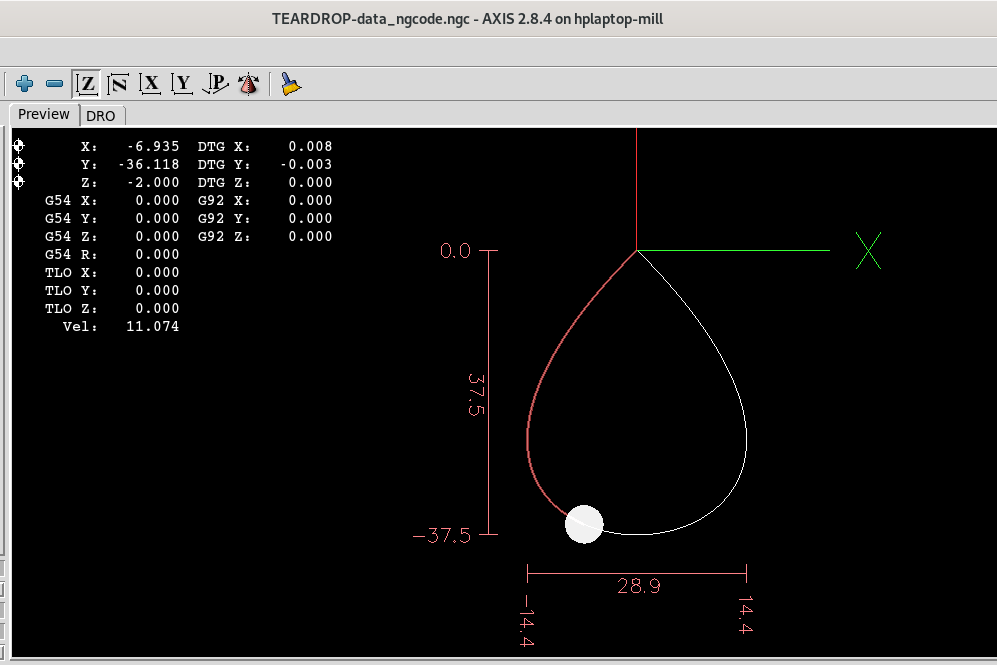
\includegraphics[width=0.565\textwidth]{./07-images/img-Ch5/TEARDROP-Axis.png}}
			 \frame{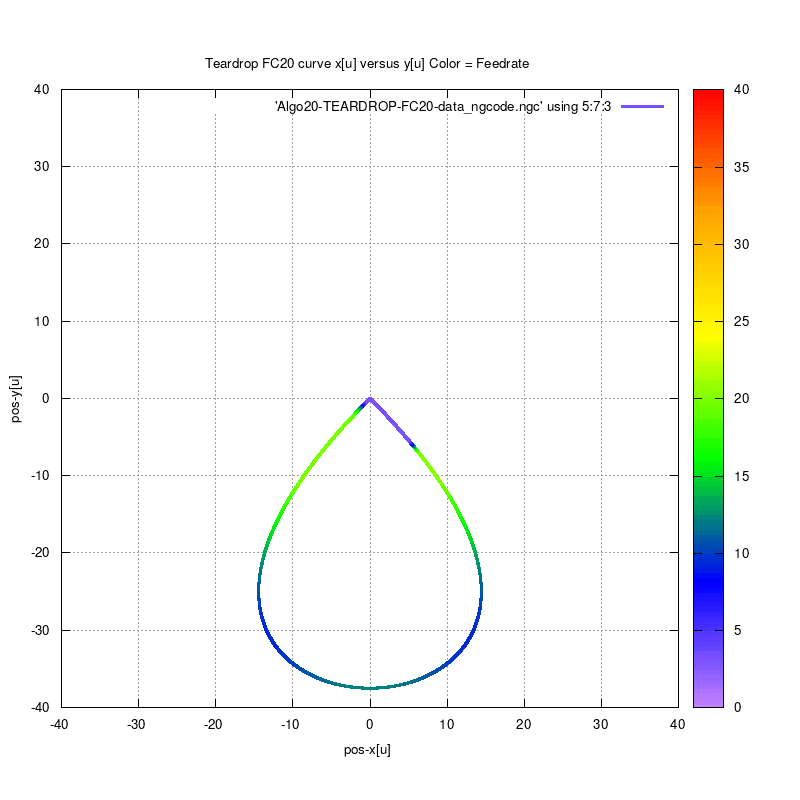
\includegraphics[width=0.38\textwidth]{./07-images/img-Ch5/TEARDROP-Feedrate.png}}\\

			\hline
		\end{tabular}
		\caption{Teardrop parametric equation and dimensions}		
		\label{table:Teardrop parametric equation}
	\end{center}
\end{table}  
